\documentclass[letterpaper, 11 pt]{article}

\usepackage{fullpage}

\usepackage{algorithmic}
\usepackage{graphics}
\usepackage{epsfig}
\usepackage{subfigure}
\usepackage{stfloats}
\usepackage{wrapfig}
%\title{\bf Proposal: Waypoint a Room with Simple Diff-Drive Robots}

\author{Kevin Kemper}

\begin{document}

\begin{flushright}
Kevin Kemper
\end{flushright}

\vspace{-2cm}
\begin{center}
\textbf{\huge ME537: Homework 2}
\end{center}


\thispagestyle{empty}
\pagestyle{empty}


%1- Precisely describe each algorithm you used and your experimental methodology. Record
%the run time, solution quality and repeatability of each approach (solve the problem at least
%10 times and provide statistical results) and discuss your results for the T10 problem.


\vspace{0.5cm}


\section{Simulated Annealing}


%\begin{wrapfigure}{r}{0.5\textwidth}
\begin{figure}[b]
	\centering
	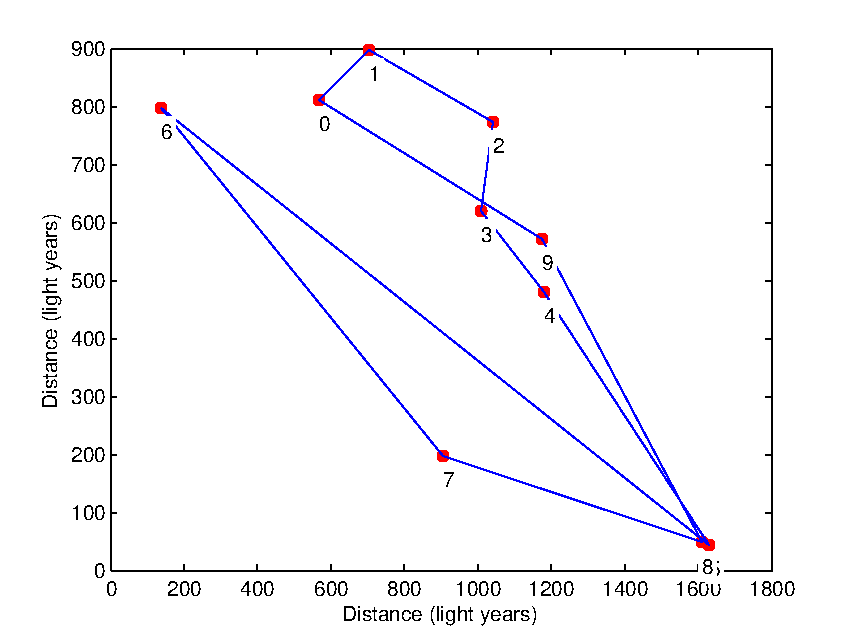
\includegraphics[scale=0.6]{../figures/path_sa_T10.pdf}
	\caption{\small	An example of a path chosen by the simulated annealing
					algorithm for 10 cities.  The dots represent city locations
					with numbers indicating the order of the visits.
			}
	\label{fig:pathsa}
%\end{wrapfigure}
\end{figure}


\[
\begin{array}{c|l}
k & \textrm{Step}\\
k_{max} & \textrm{Maximum number of steps}\\
s & \textrm{State - a path}\\
s_{best} & \textrm{Best known path}\\
s_{new} & \textrm{New path to check}\\
e & \textrm{energy - length of path}\\
e_{best} & \textrm{Length of best path}\\
e_{new} & \textrm{Length of new path}\\
T & \textrm{Temperature - a path}\\
\end{array}\]

\[
\begin{array}{c|l}
random() & \textrm{Returns random number between 0 and 1}\\
neighbor(s) & \textrm{Shuffles two adjacent cities in }s\\
energy(s) & \textrm{Returns the length of }s\\
\end{array}\]

\begin{algorithmic}
\STATE $s \gets shuffl(cities)$
\STATE $s_{best} \gets s_0$
\STATE $e \gets \infty$
\STATE $e_{best} \gets \infty$
\STATE $T \gets 1000$
\STATE $k \gets 0$
\STATE $k_{max} \gets 500$

\WHILE {$k < k_{max}$} 
		\STATE $s_{new} \gets neighbor(s)$
		\STATE $e_{new} \gets energy(s_{new})$
		
		\IF{$e_{new} < e_{best}$}
			\STATE $s_{best} \gets s_{new}$
			\STATE $e_{best} \gets e_{new}$
		\ENDIF

		\IF{$ \frac{e^{e-e_{new}}}{T} > random()$}
			\STATE $s \gets s_{new}$
			\STATE $e \gets e_{new}$
		\ENDIF
		\STATE $T \gets T \frac{kMax-k}{kMax}$
		\STATE $k \gets k + 1$
		
\ENDWHILE
\end{algorithmic}



\section{Evolutionary Algorithm}

%\begin{wrapfigure}{r}{0.5\textwidth}
\begin{figure}[b]
	\centering
	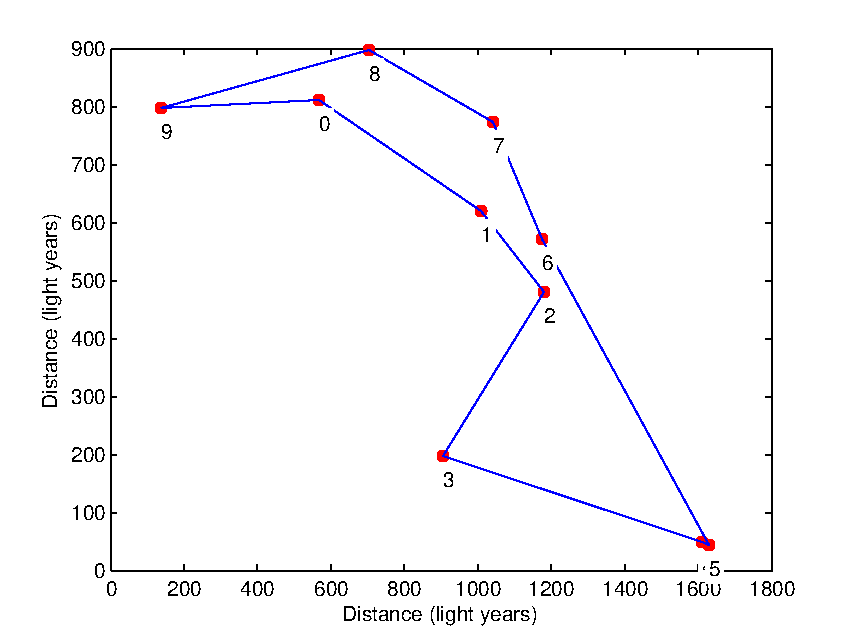
\includegraphics[scale=0.6]{../figures/path_evo_T10.pdf}
	\caption{\small	An example of a path chosen by the evolutionary algorithm
					for 10 cities.  The dots represent city locations with 
					numbers indicating the order of the visits.
			}
	\label{fig:pathevo}
%\end{wrapfigure}
\end{figure}


\[
\begin{array}{c|l}
\epsilon & \textrm{Probability of choosing a random path}\\
k & \textrm{Step}\\
k_{max} & \textrm{Maximum number of steps}\\
pop[] & \textrm{Population of possible paths}\\
s & \textrm{State - a path}\\
s_{new} & \textrm{New path to check}\\
e & \textrm{energy - length of path}\\
e_{new} & \textrm{Length of new path}\\
\end{array}\]

\[
\begin{array}{c|l}
random() & \textrm{Returns random number between 0 and 1}\\
random(pop) & \textrm{Returns a random path in the population}\\
neighbor(s) & \textrm{Shuffles two adjacent cities in }s\\
cost(s) & \textrm{Returns the length of }s\\
shuffle(cities) & \textrm{Shuffles the list of cities to genearate a random path}\\
worst(pop) & \textrm{Returns the worst in the population}\\
best(pop) & \textrm{Returns the best in the population}\\
\end{array}\]


\begin{algorithmic}

\WHILE{$i<population\ size$}
	\STATE $pop[i] \gets shuffle(cities)$
\ENDWHILE

\STATE $\epsilon \gets 0.1$
\STATE $k \gets 0$
\STATE $k_{max} \gets 500$

\WHILE {$k < k_{max}$}

		\IF{$(1-\epsilon) < random()$}
			\STATE $s_{new} \gets best(pop)$
		\ELSE
			\STATE $s_{new} \gets random(pop)$
		\ENDIF
		
		\STATE $s_{new} \gets neighbor(s_{new})$
		
		\STATE $e_{new} \gets cost(s_{new})$
		
		\IF{$eNew < cost(worst(pop))$}
			\STATE $s[worst(pop)] \gets s_{new}$
		\ENDIF

		\STATE $k \gets k + 1$
		
\ENDWHILE
\end{algorithmic}











% eta=0.026 converged slightly slower but ended with much tighter variance between trials.

%perhaps over more epochs eta of 0.001 could have converged to a better set of weights.

\begin{figure}[bt]
	\centering
	\subfigure[]{\label{fig:hTr}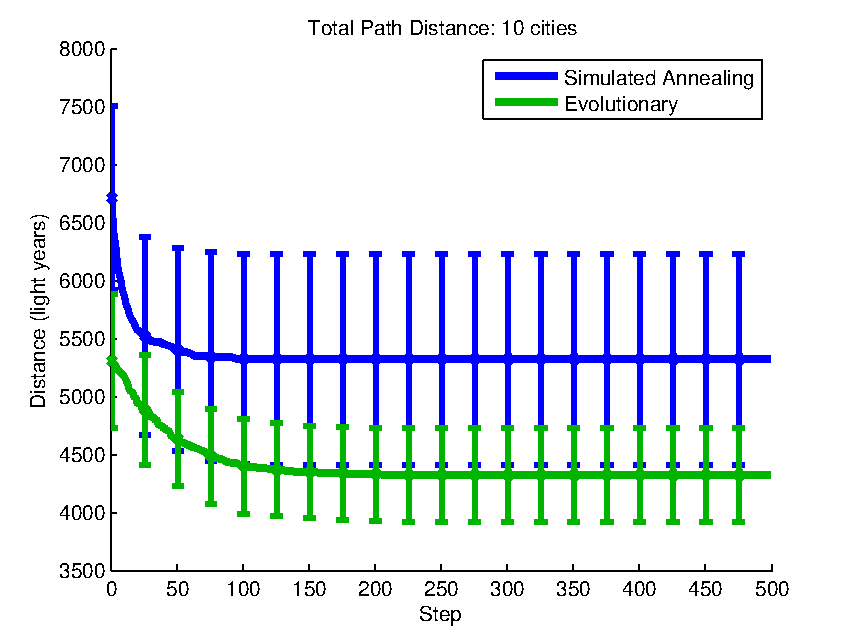
\includegraphics[scale=1]{../figures/out_T10.pdf}}
	\subfigure[]{\label{fig:hT1}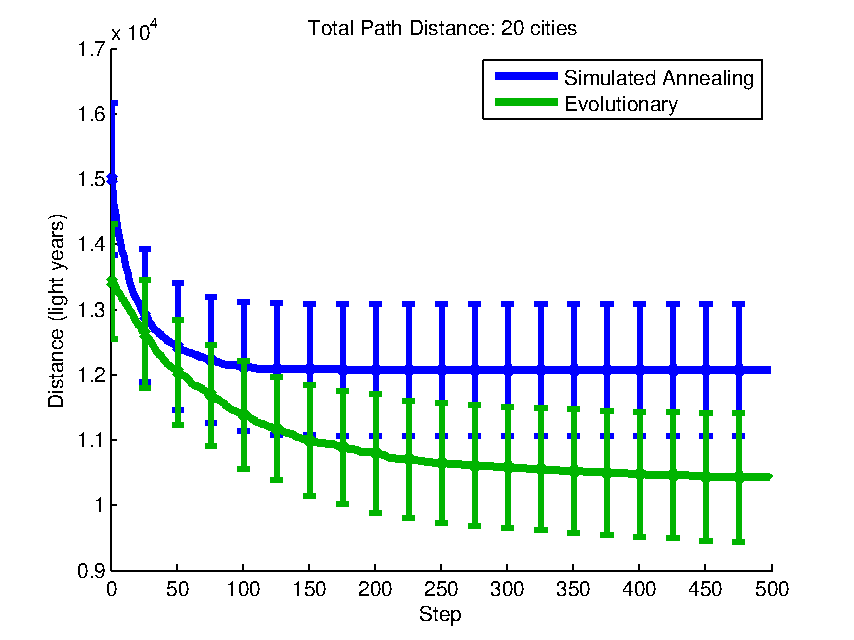
\includegraphics[scale=1]{../figures/out_T20.pdf}}
	\caption{	Performance of simulated annealing vs. an evolutionary algorithm.}
	\label{fig:h1}
\end{figure}

\begin{figure}[bt]
	\centering
	\subfigure[]{\label{fig:hT2}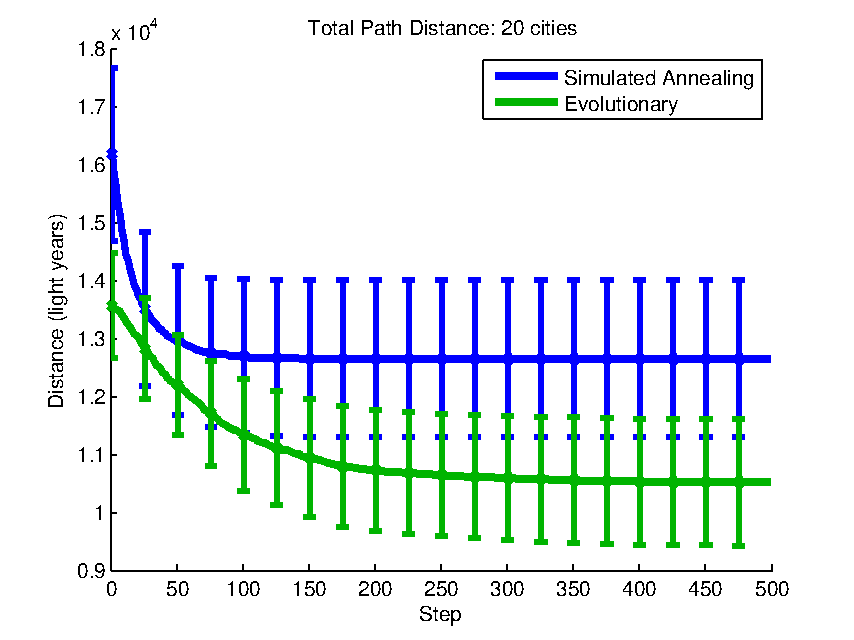
\includegraphics[scale=1]{../figures/out_T20A.pdf}}
	\subfigure[]{\label{fig:hT3}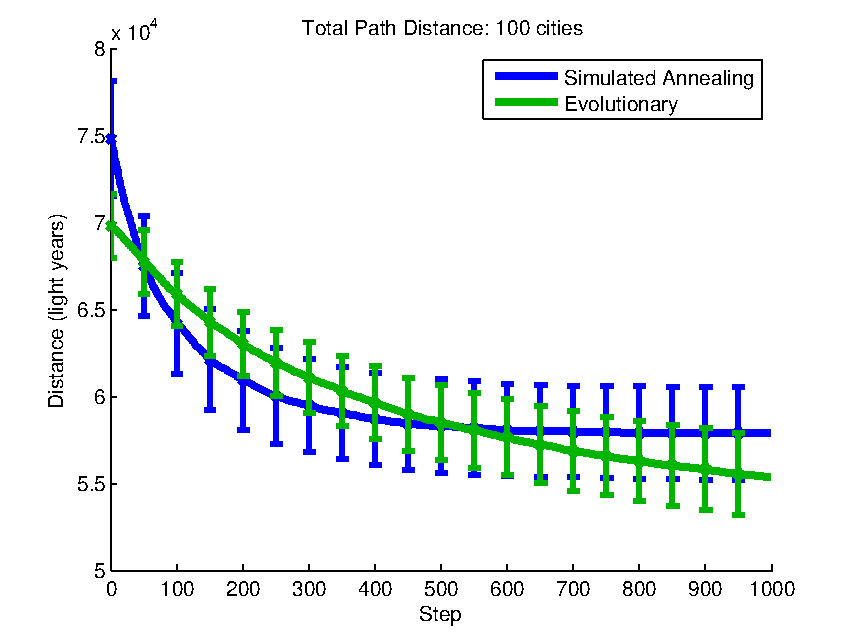
\includegraphics[scale=1]{../figures/out_T100.pdf}}
	\caption{	Performance of simulated annealing vs. an evolutionary algorithm.}
	\label{fig:h2}
\end{figure}




\end{document}
